\documentclass[DaoFP]{subfiles}
\begin{document}
\setcounter{chapter}{17}

\chapter{端与余端}

\section{Profunctors(函子)}

在范畴论的高深领域中,我们遇到了一些模式,这些模式与它们的起源相距甚远,以至于我们难以形象化它们。更糟糕的是,模式越抽象,其具体示例之间的差异就越大。

从$a$到$b$的箭头相对容易形象化。我们有一个非常熟悉的模型:一个消耗$a$的元素并生成$b$的元素的函数。Hom-set(同态集)是这些箭头的集合。

函子是范畴之间的箭头。它消耗一个范畴中的对象和箭头,并生成另一个范畴中的对象和箭头。我们可以将其视为从源范畴提供的材料构建这些对象(和箭头)的配方。特别是,我们通常将自函子视为建筑材料的容器。

Profunctor(函子)将一对对象$\langle a, b \rangle$映射到一个集合$P\langle a, b \rangle$,并将一对箭头:
\[ \langle f \colon s \to a, g \colon b \to t \rangle \]
映射到一个函数:
\[ P\langle f, g \rangle \colon P\langle a, b \rangle \to P\langle s, t \rangle\]

Profunctor是一种抽象,它结合了许多其他抽象的元素。由于它是一个函子$ \mathcal{C}^{op} \times  \mathcal{C} \to \mathbf{Set}$,我们可以将其视为从一对对象构建一个集合,并从一对箭头(其中一个箭头方向相反)构建一个函数。然而,这并没有帮助我们的想象力。

幸运的是,我们有一个很好的Profunctor模型:hom-functor(同态函子)。当对象变化时,两个对象之间的箭头集合表现得像一个Profunctor。同样,变化hom-set的源和目标之间的差异也是有意义的。

因此,我们可以将任意Profunctor视为hom-functor的推广。Profunctor在已有的hom-sets之上提供了对象之间的额外桥梁。

然而,hom-set $ \mathcal{C}(a, b)$的元素和集合$P\langle a, b \rangle$的元素之间有一个很大的区别。hom-set的元素是箭头,而箭头可以组合。如何组合Profunctors并不立即显而易见。

诚然,Profunctor对箭头的提升可以视为组合的推广——只是不是在Profunctors之间,而是在hom-sets和Profunctors之间。例如,我们可以用箭头$f \colon s \to a$“预组合”$P \langle a, b \rangle$,得到$P \langle s, b \rangle$:
\[ P\langle f, id_b \rangle \colon P \langle a, b \rangle \to P \langle s, b \rangle \]
同样,我们可以用$g \colon b \to t$“后组合”它:
\[ P \langle id_a, g \rangle \colon P \langle a, b \rangle \to P \langle a, t \rangle \]
这种异质组合接受一个由箭头和Profunctor元素组成的可组合对,并生成一个Profunctor元素。

Profunctor可以通过提升一对箭头在两侧进行扩展:

\[
 \begin{tikzcd}
  & s
  \arrow[r, bend left, dashed, blue, "f"]
 & a
 \arrow[r, bend right, "P"]
 & b
  \arrow[r, bend left, dashed, blue, "g"]
 &  t
  \end{tikzcd}
\]

\subsection{Collages(拼贴)}

没有理由将Profunctor限制在单一范畴中。我们可以轻松地将两个范畴之间的Profunctor定义为函子$ P \colon \mathcal{C}^{op} \times  \mathcal{D} \to \mathbf{Set}$。这样的Profunctor可以通过生成从$\mathcal{C}$中的对象到$\mathcal{D}$中的对象的缺失的hom-sets来将两个范畴粘合在一起。

两个范畴$\mathcal{C}$和$\mathcal{D}$的拼贴(或\index{cograph}余图)是一个范畴,其对象来自两个范畴(一个不相交的并集)。两个对象$x$和$y$之间的hom-set要么是$\mathcal{C}$中的hom-set,如果两个对象都在$\mathcal{C}$中;要么是$\mathcal{D}$中的hom-set,如果两个对象都在$\mathcal{D}$中;要么是集合$P \langle x, y\rangle$,如果$x$在$\mathcal{C}$中且$y$在$\mathcal{D}$中。否则,hom-set为空。

态射的组合是通常的组合,除非其中一个态射是$P \langle x, y \rangle$的元素。在这种情况下,我们提升我们试图预组合或后组合的态射。

很容易看出,拼贴确实是一个范畴。拼贴两侧之间的新态射有时被称为\index{heteromorphism}异态射。它们只能从$\mathcal{C}$到$\mathcal{D}$,而不能反过来。

这样看来,Profunctor $ \mathcal{C}^{op} \times  \mathcal{C} \to \mathbf{Set}$应该真正被称为\emph{自}-Profunctor。它定义了$\mathcal{C}$与自身的拼贴。

\begin{exercise}
证明存在一个从两个范畴的拼贴到“行走箭头”范畴的函子,该范畴有两个对象和一个箭头(以及两个恒等箭头)。
\end{exercise}
\begin{exercise}
证明如果存在一个从$\mathcal{C}$到行走箭头范畴的函子,那么$\mathcal{C}$可以被拆分为两个范畴的拼贴。
\end{exercise}

\subsection{Profunctors作为关系}

在显微镜下,Profunctor看起来像hom-functor,集合$P \langle a, b \rangle$的元素看起来像单个箭头。但当我们放大时,我们可以将Profunctor视为对象之间的关系。这些不是通常的关系;它们是\index{proof-relevant relation}\emph{证明相关}的关系。

为了更好地理解这个概念,让我们考虑一个常规函子$F \colon \mathcal{C} \to \mathbf{Set}$(换句话说,一个协预层)。一种解释它的方式是,它定义了$\mathcal{C}$对象的一个\index{proof-relevant subset}子集,即那些被映射到非空集合的对象。$F a$的每个元素都被视为$a$是这个子集成员的证明。另一方面,如果$F a$是一个空集,那么$a$不是这个子集的成员。

我们可以将相同的解释应用于Profunctors。如果集合$P \langle a, b \rangle$为空,我们说$b$与$a$无关。如果它不为空,我们说集合$P \langle a, b \rangle$的每个元素都代表$b$与$a$相关的证明。然后,我们可以将Profunctor视为一个证明相关的关系。

请注意,我们不对这个关系做任何假设。它不必是自反的,因为$P \langle a, a \rangle$可能为空(事实上,$P \langle a, a \rangle$仅对自Profunctors有意义)。它也不必是对称的。

由于hom-functor是(自)Profunctor的一个例子,这种解释让我们以新的视角看待hom-functor:作为范畴中对象之间内置的证明相关关系。如果两个对象之间存在箭头,则它们是相关的。请注意,这种关系是自反的,因为$\mathcal{C}(a, a)$永远不会为空:至少它包含恒等态射。

此外,正如我们之前所见,hom-functors与Profunctors相互作用。如果$a$通过$P$与$b$相关,并且hom-sets $\mathcal{C}(s, a)$和$\mathcal{D}(b, t)$非空,那么自动地$s$通过$P$与$t$相关。因此,Profunctors是与它们操作的范畴结构兼容的证明相关关系。

我们知道如何将Profunctor与hom-functors组合,但如何组合两个Profunctors呢?我们可以从关系的组合中得到线索。

假设你想给手机充电,但没有充电器。为了将你连接到充电器,只要有一个拥有充电器的朋友就足够了。任何朋友都可以。你将拥有朋友的关系与拥有充电器的人的关系组合起来,得到能够给手机充电的关系。你能给手机充电的证明是一对证明,一个是友谊的证明,另一个是拥有充电器的证明。

一般来说,我们说两个对象通过复合关系相关,如果存在一个中间对象与它们两者都相关。

\subsection{Haskell中的Profunctor组合}

关系的组合可以转化为Haskell中的Profunctor组合。让我们首先回顾Profunctor的定义:
\begin{haskell}
class Profunctor p where
  dimap :: (s -> a) -> (b -> t) -> (p a b -> p s t)
\end{haskell}

理解Profunctor组合的关键在于它需要中间对象的\emph{存在}。对于对象$b$通过复合$P \diamond Q$与对象$a$相关,必须存在一个对象$x$来弥合差距:
\[
 \begin{tikzcd}
  & a
  \arrow[r, bend left, blue, "Q"]
 & x
  \arrow[r, bend left, red, "P"]
 & b
  \end{tikzcd}
\]

这可以在Haskell中使用存在类型进行编码。给定两个Profunctors \hask{p}和\hask{q},它们的组合是一个新的Profunctor \hask{Procompose p q}:
\begin{haskell}
data Procompose p q a b where
  Procompose ::  q a x -> p x b -> Procompose p q a b
\end{haskell}
我们使用\hask{GADT}来表达对象\hask{x}的存在性。数据构造函数的两个参数可以看作是一对证明:一个证明\hask{x}与\hask{a}相关,另一个证明\hask{b}与\hask{x}相关。这对证明构成了\hask{b}与\hask{a}相关的证明。

存在类型可以看作和类型(sum type)的推广。我们对所有可能的类型\hask{x}求和。就像有限和可以通过注入其中一个替代项来构造(想想\hask{Either}的两个构造函数),存在类型可以通过为\hask{x}选择特定类型并将其注入\hask{Procompose}的定义来构造。

正如从和类型映射出来需要一对函数,每个替代项一个;从存在类型映射出来需要一个函数族,每个类型一个。例如,从\hask{Procompose}映射出来由一个多态函数给出:
\begin{haskell}
mapOut :: Procompose p q a b -> (forall x. q a x -> p x b -> c) -> c
mapOut (Procompose qax pxb) f = (f qax pxb)
\end{haskell}

Profunctors的组合再次是一个Profunctor,可以从以下实例中看出:
\begin{haskell}
instance (Profunctor p, Profunctor q) => Profunctor (Procompose p q) 
  where
    dimap l r (Procompose qax pxb) = 
               Procompose (dimap l id qax) (dimap id r pxb)
\end{haskell}
这只是说你可以通过将第一个Profunctor向左扩展,第二个Profunctor向右扩展来扩展复合Profunctor。

这个Profunctor组合的定义在Haskell中有效是由于参数性。语言以某种方式限制了Profunctors的类型,使得这个定义有效。然而,一般来说,对中间对象进行简单的求和会导致过度计数,因此在范畴论中我们必须对此进行补偿。

\section{余端(Coends)}

在朴素定义profunctors(profunctor,也称为分布函子)的复合时,过度计数的问题发生在两个中间对象候选通过一个态射连接时:
\[
 \begin{tikzcd}
  & a
  \arrow[r, bend left, blue, "Q"]
  &x
  \arrow[r, dashed, "f"]
 & y
  \arrow[r, bend left, red, "P"]
 & b
  \end{tikzcd}
\]
我们可以通过在右侧扩展$Q$,通过提升$Q \langle id, f \rangle$,并使用$y$作为中间对象;或者我们可以在左侧扩展$P$,通过提升$P \langle f, id \rangle$,并使用$x$作为中介。

为了避免双重计数,我们必须在应用于profunctors时调整我们对和类型的定义。由此产生的构造称为余端(coend)。

首先,让我们重新表述这个问题。我们试图在乘积中对所有对象$x$求和:
\[ P \langle a, x \rangle \times Q \langle x, b \rangle \]
双重计数的发生是因为我们可以在两个profunctors之间打开一个间隙,只要有一个态射可以插入其中。因此,我们实际上是在看一个更一般的乘积:
\[ P \langle a, x \rangle \times Q \langle y, b \rangle \]
重要的观察是,如果我们固定端点$a$和$b$,这个乘积是一个关于$\langle y, x \rangle$的profunctor。通过一些重排(在同构意义上)可以很容易地看到这一点:
\[ Q \langle y, b \rangle \times P \langle a, x \rangle \]
我们感兴趣的是这个profunctor的对角线部分的和,即当$x$等于$y$时。

因此,让我们看看如何定义一般profunctor $P$的所有对角线项的和。事实上,这个构造适用于任何函子$P \colon \cat C^{op} \times \cat C \to D$,而不仅仅是$\Set$值的profunctors。

对角线对象的和由注入定义;在这种情况下,每个$\cat C$中的对象都有一个注入。这里我们只展示其中两个,以及代表所有其他注入的虚线:
\[
 \begin{tikzcd}
 P \langle y, y \rangle
 \arrow[dr, "i_y"']
 \arrow[rr, dash, dashed]
 &&P \langle x, x \rangle
 \arrow[dl, "i_x"]
 \\
 & d
 \end{tikzcd}
\]

如果我们在定义一个和,我们会使其成为一个具有这些注入的通用对象。但由于我们处理的是两个变量的函子,我们希望通过“扩展”某个共同祖先来识别相关的注入——在这里,$P \langle y, x \rangle$。我们希望以下图表在任何连接态射$f\colon x \to y$存在时交换:

\[
 \begin{tikzcd}
 &P \langle y, x \rangle
 \arrow[ld, "{P \langle id, f \rangle}"']
 \arrow[rd, "{P \langle f, id \rangle}"]
 \\
 P \langle y, y \rangle
 \arrow[dr, "i_y"']
 &&P \langle x, x \rangle
 \arrow[dl, "i_x"]
 \\
 &d
 \end{tikzcd}
\]
这个图表被称为\index{余楔}余楔(co-wedge),其交换条件称为余楔条件。对于每个$f \colon x \to y$,我们要求:
\[ i_x \circ P \langle f, id_y \rangle = i_y \circ P \langle id_x, f \rangle \]
\emph{通用}余楔称为余端(coend)。

由于余端将和推广到可能无限的域,我们使用积分符号来表示它,并将“积分变量”放在顶部:
\[ \int^{x\colon \mathcal{C}} P \langle x, x \rangle \]
通用性意味着,每当$\cat D$中有一个对象$d$配备了一族满足余楔条件的箭头$g_x \colon P \langle x, x \rangle \to d$时,存在一个从余端到$d$的唯一映射:
\[ h \colon \int^{x\colon \mathcal{C}} P \langle x, x \rangle \to d \]
它通过注入$i_x$分解每个$g_x$:
\[ g_x = h \circ i_x \]
图示如下:
\[
 \begin{tikzcd}
 &P \langle y, x \rangle
 \arrow[ld, "{P \langle id, f \rangle}"']
 \arrow[rd, "{P \langle f, id \rangle}"]
 \\
 P \langle y, y \rangle
 \arrow[dr, "i_y"']
 \arrow[ddr, bend right,  "g_y"']
 &&P \langle x, x \rangle
 \arrow[dl, "i_x"]
 \arrow[ddl, bend left,  "g_x"]
 \\
 &\int^x P \langle x, x \rangle
 \arrow[d, dashed, "h"]
 \\
 &d
 \end{tikzcd}
\]

将其与两个对象的和的定义进行比较:

\[
 \begin{tikzcd}
 a
 \arrow[dr, "\text{Left}"]
 \arrow[ddr, bend right, "f"']
 && b
 \arrow[dl, "\text{Right}"']
 \arrow[ddl, bend left, "g"]
 \\
&a + b
\arrow[d, dashed, "h"]
\\
& d
 \end{tikzcd}
\]
正如和被定义为通用余楔,余端被定义为通用余楔。

特别是,如果你要构造一个$\Set$值的profunctor的余端,你会从所有集合$P \langle x, x \rangle$的和(一个区分并集)开始。然后你会识别满足余楔条件的这个和的所有元素。每当存在一个元素$c  \in P \langle y, x \rangle$和一个态射$f \colon x \to y$时,你会将元素$a \in P \langle x, x \rangle$与元素$b \in P \langle y, y \rangle$识别为:
\[ P \langle id, f \rangle (c) = b\]
和
\[ P \langle f, id \rangle (c) = a\]

注意,在离散范畴(即没有箭头连接的对象集合)中,余楔条件是平凡的(除了恒等态射外没有其他$f$),因此余端只是对角线对象$P \langle x, x \rangle$的简单和(余积)。

\subsection{外自然变换(Extranatural transformations)}

目标范畴中由源范畴对象参数化的一族箭头通常可以组合成两个函子之间的单个自然变换。

我们在余楔定义中的注入形成了一族由对象参数化的函数,但它们并不完全符合自然变换的定义。
\[
 \begin{tikzcd}
 P \langle y, y \rangle
 \arrow[dr, "i_y"']
 \arrow[rr, dash, dashed]
 &&P \langle x, x \rangle
 \arrow[dl, "i_x"]
 \\
 &d
 \end{tikzcd}
\]
问题在于函子$P \colon \cat C^{op} \times \cat C \to \cat D$在第一个参数中是反变的,在第二个参数中是协变的;因此其对角线部分,在对象上定义为$x \mapsto P \langle x, x \rangle$,既不是反变的也不是协变的。

我们手头最接近的自然性类比是余楔条件:
\[
 \begin{tikzcd}
 &P \langle y, x \rangle
 \arrow[ld, "{P \langle id, f \rangle}"']
 \arrow[rd, "{P \langle f, id \rangle}"]
 \\
 P \langle y, y \rangle
 \arrow[dr, "i_y"']
 &&P \langle x, x \rangle
 \arrow[dl, "i_x"]
 \\
 &d
 \end{tikzcd}
\]
确实,与自然性方块一样,它涉及态射$f \colon x \to y$的提升(在这里以两种不同的方式)与变换$i$的分量之间的交互。

当然,标准的自然性条件处理的是成对的函子。在这里,变换的目标是一个固定对象$d$。但我们总是可以将其重新解释为常数profunctor $\Delta_d \colon \cat C^{op} \times \cat C \to \cat D$的输出。因此,为了推广自然性,我们用任意profunctor $Q$替换$\Delta_d$。

我们将余楔条件重新解释为更一般的\index{外自然变换}\emph{外自然}变换的特殊情况。外自然变换是一族箭头:
\[ \alpha_{c d} \colon P \langle c, c \rangle \to Q \langle d, d \rangle \]
在两个形式如下的函子之间:
\[ P \colon \cat C^{op} \times \cat C \to \cat E \]
\[ Q \colon \cat D^{op} \times \cat D \to \cat E \]
在$c$中的外自然性意味着对于任何态射$f \colon c \to c'$,以下图表交换:
\[
 \begin{tikzcd}
 &P \langle c', c \rangle
 \arrow[ld, "{P \langle id, f \rangle}"']
 \arrow[rd, "{P \langle f, id \rangle}"]
 \\
      P \langle c', c' \rangle
 \arrow[dr, "\alpha_{c' d}"']
 &&P \langle c, c \rangle
 \arrow[dl, "\alpha_{c d}"]
 \\
 & Q \langle d, d \rangle
 \end{tikzcd}
\]
在$d$中的外自然性意味着对于任何态射$g \colon d \to d'$,以下图表交换:
\[
 \begin{tikzcd}
 &P \langle c, c \rangle
 \arrow[ld, "\alpha_{c d}"']
 \arrow[rd, "\alpha_{c d'}"]
 \\
      Q \langle d, d \rangle
 \arrow[dr, "{Q \langle id, g\rangle}"']
 &&Q \langle d', d' \rangle
 \arrow[dl, "{Q \langle g,  id\rangle}"]
 \\
 & Q \langle d, d' \rangle
 \end{tikzcd}
\]

根据这个定义,我们得到余楔条件作为profunctor $P$与常数profunctor $\Delta_d$之间的外自然性。

我们现在可以将余端的定义重新表述为一对$(c, i)$,其中$c$是配备有外自然变换$i \colon P \to \Delta_c$的对象,该变换在所有这样的对中是通用的。

通用性意味着对于任何配备有外自然变换$\alpha \colon P \to \Delta_d$的对象$d$,存在一个唯一态射$h \colon c \to d$,它通过$i$的分量分解$\alpha$的所有分量:
\[ \alpha_x = h \circ i_x \]
我们称这个对象$c$为余端,并将其写为:
\[ c = \int^x P\langle x, x \rangle \]

\begin{exercise}
验证对于外自然变换$P \to \Delta_d$,第一个外自然性菱形等价于余楔条件,第二个是平凡满足的。
\end{exercise}

\subsection{使用余端的Profunctor复合}

有了余端的定义,我们现在可以正式定义两个profunctors的复合:

\[ (P \diamond Q)\langle a, b \rangle = \int^{x\colon \mathcal{C}} Q \langle a, x \rangle \times P \langle x, b \rangle\]
将其与以下Haskell代码进行比较:
\begin{haskell}
data Procompose p q a b where
  Procompose ::  q a x -> p x b -> Procompose p q a b
\end{haskell}

在Haskell中我们不必担心余楔条件的原因类似于所有参数多态函数自动满足自然性条件的原因。余端是使用一族注入定义的;在Haskell中,所有这些注入都是由一个\emph{单一}的多态函数定义的:
\begin{haskell}
data Coend p where
  Coend ::  p x x -> Coend p
\end{haskell}
\index{参数性}参数性(Parametricity)然后强制执行余楔条件。

余端在处理profunctors时引入了一个新的抽象层次。使用余端的计算通常利用它们的映射出属性。要定义一个从余端到某个对象$d$的映射:
\[ \int^x P \langle x, x \rangle \to d \]
只需定义一族从函子的对角线项到$d$的函数:
 \[ g_x \colon P \langle x, x \rangle \to d \]
 满足余楔条件。你可以从这个技巧中获得很多好处,特别是与Yoneda引理结合时。我们将在接下来的内容中看到这方面的例子。

\begin{exercise}
为以下profunctor对定义\hask{Profunctor}实例:
\begin{haskell}
newtype ProPair q p a b x y = ProPair (q a y, p x b)
\end{haskell}
提示:保持前四个参数固定:
\begin{haskell}
instance (Profunctor p, Profunctor q) => Profunctor (ProPair q p a b)
\end{haskell}
\end{exercise}

\begin{exercise}
Profunctor复合可以使用余端表示:
\begin{haskell}
newtype CoEndCompose p q a b = CoEndCompose (Coend (ProPair q p a b))
\end{haskell}
为\hask{CoEndCompose}定义\hask{Profunctor}实例。
\end{exercise}

\subsection{余极限作为余端}
忽略其中一个变量的双变量函数等价于单变量函数。类似地,忽略其中一个变量的profunctor等价于一个函子。反之,给定一个函子$F$,我们可以构造一个平凡的profunctor。其在对象上的作用由下式给出:
\[P \langle x, y \rangle = F y \]
其在一对箭头上的作用忽略其中一个箭头:
\[P \langle f, g \rangle = F g \]

对于任何$f \colon x \to y$,我们对此类profunctor的余端定义简化为以下图表:
\[
 \begin{tikzcd}
 & F x
 \arrow[ld, "F f"']
 \arrow[rd, dashed, "id_{F x}"]
 \\
 F y
 \arrow[dr, "i_y"']
 \arrow[ddr, bend right,  "g_y"']
 && F x
 \arrow[dl, "i_x"]
 \arrow[ddl, bend left,  "g_x"]
 \\
 &\int^x F x
 \arrow[d, dashed, "h"]
 \\
 &d
 \end{tikzcd}
\]
在缩小恒等箭头后,原始的余楔变为余锥,通用条件变为余极限的定义。这证明了使用余端符号表示余极限的合理性:
\[ \int^x F x = \text{colim} F \]
函子$F$定义了目标范畴中的一个图表。模式是整个源范畴。

如果我们考虑离散范畴,我们可以获得有用的直觉,其中profunctor是一个(可能是无限的)矩阵,余端是其对角线元素的和(余积)。沿一个轴为常数的profunctor对应于一个行相同的矩阵(每行由“向量”$F x$给出)。此类矩阵的对角线元素的和等于向量$F x$的所有分量的和。
\[
\begin{pmatrix}
\color{red} F a & F b & F c & ... \\
F a & \color{red}F b & F c & ...\\
F a & F b &\color{red}F c & ...\\
... & ... & ... & ...
\end{pmatrix}
\]
在非离散范畴中,这个和推广为余极限。

\section{Ends}

正如余end(coend)推广了profunctor对角元素的和——它的对偶,end推广了积。积由其投影定义,end也是如此。

我们在积的定义中使用的span的推广将是一个对象$d$,带有一族投影,每个对象$x$对应一个:
\[ \pi_x \colon d \to P \langle x, x \rangle \]
余楔(co-wedge)的对偶称为\index{wedge}楔(wedge):
\[
 \begin{tikzcd}
 &d
 \arrow[ld, "\pi_x"']
 \arrow[rd, "\pi_y"]
 \\
 P \langle x, x \rangle
 \arrow[dr, "{P \langle id, f \rangle}"']
 &&P \langle y, y \rangle
 \arrow[dl, "{P \langle f, id \rangle}"]
 \\
 & P \langle x, y \rangle
 \end{tikzcd}
\]
对于每个箭头$f \colon x \to y$,我们要求:
\[ P \langle f, id_y \rangle \circ \pi_y = P \langle id_x, f \rangle \circ \pi_x \]

end是一个泛楔(universal wedge)。我们也用积分符号表示它,这次将“积分变量”放在底部。
\[ \int_{x \colon \cat C} P \langle x, x \rangle \]

你可能会好奇,为什么在微积分中,基于乘法而不是加法的积分很少使用。这是因为我们总是可以使用对数将乘法替换为加法。在范畴论中我们没有这种便利,因此end和coend同样重要。

总结一下,end是一个配备有一族态射(投影)的对象:
\[ \pi_a \colon \left( \int_x P \langle x, x \rangle \right) \to P \langle a, a \rangle \]
满足楔条件。

它在这些对象中是泛的;也就是说,对于任何其他配备有一族箭头$g_x$并满足楔条件的对象$d$,存在一个唯一的态射$h$,使得族$g_x$通过族$\pi_x$分解:
\[ g_x = \pi_x \circ h \]
图示如下:
\[
 \begin{tikzcd}
 &d
 \arrow[ddl, bend right, "g_x"']
 \arrow[ddr, bend left, "g_y"]
 \arrow[d, dashed, "h"]
 \\
 & \int_x P \langle x, x \rangle
 \arrow[ld, "\pi_x"']
 \arrow[rd, "\pi_y"]
 \\
 P \langle x, x \rangle
 \arrow[dr, "{P \langle id, f \rangle}"']
 &&P \langle y, y \rangle
 \arrow[dl, "{P \langle f, id \rangle}"]
 \\
 & P \langle x, y \rangle
 \end{tikzcd}
\]

等价地,我们可以说end是一个由对象$e = \int_x P\langle x, x\rangle$和一个\index{extranatural transformation}外自然变换(extranatural transformation)$\pi \colon \Delta_d \to e$组成的对$(e, \pi)$,它在这些对中是泛的。楔条件实际上是外自然性条件的一个特例。

如果你要构造一个$\Set$值profunctor的end,你会从范畴$\cat C$中所有对象的$P \langle x, x \rangle$的巨型积开始,然后剔除不满足楔条件的元组。

特别地,想象用单元素集$1$代替$d$。族$g_x$会从每个集合$P \langle x, x \rangle$中选择一个元素。这将给你一个巨型元组。你会剔除大部分这些元组,只留下满足楔条件的那些。

再次,在Haskell中,由于\index{parametricity}参数性(parametricity),楔条件自动满足,profunctor \hask{p}的end的定义简化为:

\begin{haskell}
type End p = forall x. p x x
\end{haskell}

Haskell中\hask{End}的实现并没有展示它是\hask{Coend}的对偶。这是因为,在撰写本文时,Haskell没有内置的存在类型语法。如果有,\hask{Coend}将实现为:
\begin{haskell}
type Coend p = exists x. p x x
\end{haskell}

\hask{Coend}和\hask{End}之间的存在/全称对偶意味着构造一个\hask{Coend}很容易——你只需要选择一个类型\hask{x},对于该类型你有一个类型\hask{p x x}的值。另一方面,要构造一个\hask{End},你必须提供一族值\hask{p x x},每个类型\hask{x}对应一个。换句话说,你需要一个由\hask{x}参数化的多态公式。多态函数的定义就是这种公式的典型例子。


\subsection{自然变换作为end}

end最有趣的应用是简洁地定义自然变换的集合。考虑两个函子$F$和$G$,它们在两个范畴$\mathcal{B}$和$\mathcal{C}$之间。它们之间的自然变换是$\mathcal{C}$中的一族箭头$\alpha_x$。你可以将其视为从每个hom集$\mathcal{C} (F x, G x)$中选取一个元素$\alpha_x$。
\[
 \begin{tikzcd}
 && F x
 \arrow[dd, "{\alpha_x \in \cat C (F x, G x)}"]
 \\
 x
 \arrow[urr, dashed, "F"]
 \arrow[drr, dashed, "G"]
 \\
 && G x
 \end{tikzcd}
\]

我们知道映射$\langle a, b \rangle \to \mathcal{C} (a, b)$定义了一个profunctor。事实证明,对于任何一对函子,映射$\langle a, b \rangle \to \mathcal{C} (F a, G b)$也表现得像一个profunctor。这个profunctor在一对箭头$\langle f \colon s \to a, g \colon b \to t \rangle$上的作用是一个函数:
\[ \cat C(F a, G b) \to \cat C (F s, G t) \]
由以下复合给出:
\[ F s \xrightarrow{F f} F a \xrightarrow{h} G b \xrightarrow{G g} G t \]
其中$h$是$\mathcal{C} (F a, G b)$中的一个元素。

这个profunctor的对角部分非常适合作为自然变换的分量。事实上,end:
\[  \int_{x \colon  \mathcal{B}} \mathcal{C}(F x, G x) \]
定义了从$F$到$G$的自然变换的集合。

为了证明这一点,让我们检查楔条件。代入我们的profunctor,我们得到:

\[
 \begin{tikzcd}
 & \int_{x} \mathcal{C}(F x, G x)
 \arrow[ld, "\pi_a"']
 \arrow[rd, "\pi_b"]
 \\
  \mathcal{C} ( F a, G a )
 \arrow[dr, "{(Ff \, \circ \, -)}"']
 && \mathcal{C} \langle F b, G b \rangle
 \arrow[dl, "{(- \, \circ\, Gf)}"]
 \\
 &  \mathcal{C} ( F a, G b )
 \end{tikzcd}
\]

我们可以通过实例化单元素集的泛条件来选取集合$\int_{x} \mathcal{C}(F x, G x)$中的一个元素:

\[
 \begin{tikzcd}
 & 1
 \arrow[d, dashed, "\alpha"]
\arrow[ddl, bend right, "\alpha_a"']
 \arrow[ddr, bend left, "\alpha_b"]
 \\
 & \int_{x} \mathcal{C}(F x, G x)
 \arrow[ld, "\pi_a"']
 \arrow[rd, "\pi_b"]
 \\
  \mathcal{C} ( F a, G a )
 \arrow[dr, "{(F f \, \circ \, -)}"']
 && \mathcal{C} ( F b, G b )
 \arrow[dl, "{(- \, \circ\, G f)}"]
 \\
 &  \mathcal{C} ( F a, G b )
 \end{tikzcd}
\]
我们从hom集$\mathcal{C} ( F a, G a )$中选取分量$\alpha_a$,从$\mathcal{C} ( F b, G b )$中选取分量$\alpha_b$。楔条件简化为:
\[ F f \circ \alpha_a = \alpha_b \circ G f \]
对于任何$f \colon a \to b$。这正是自然性条件。因此,这个end的任何元素$\alpha$自动是一个自然变换。

因此,自然变换的集合,或函子范畴中的hom集,由end给出:
\[ [\mathcal{C}, \mathcal{D}] (F, G) \cong \int_{x \colon  \mathcal{B}} \mathcal{C}(F x, G x)\]

在Haskell中,这与我们之前的定义一致:
\begin{haskell}
type Natural f g = forall x. f x -> g x
\end{haskell}

正如我们之前讨论的,要构造一个\hask{End},我们必须给它一族由类型参数化的值。在这里,这些值是多态函数的分量。

\subsection{极限作为ends}
正如我们能够将余极限(colimits)表示为coends,我们也可以将极限(limits)表示为ends。和之前一样,我们定义一个忽略其第一个参数的平凡profunctor:
\begin{align*}
 P \langle x, y \rangle &= F y \\
 P \langle f, g \rangle &= F g 
\end{align*}
定义end的泛条件变成了泛锥(universal cone)的定义:
\[
 \begin{tikzcd}
 &d
 \arrow[ddl, bend right, "g_x"']
 \arrow[ddr, bend left, "g_y"]
 \arrow[d, dashed, "h"]
 \\
 & \int_x F x
 \arrow[ld, "\pi_x"']
 \arrow[rd, "\pi_y"]
 \\
 F x
 \arrow[dr, "F f"']
 &&F y
 \arrow[dl, dashed, "id_{F y}"]
 \\
 & F y
 \end{tikzcd}
\]
因此,我们可以使用end符号表示极限:
\[ \int_x F x = \text{lim} F \]

\begin{exercise}
积是一个从二对象范畴$\Cat 2$出发的函子的极限。证明它可以定义为一个end。提示:$\Cat 2$中没有非恒等态射。
\end{exercise}

\section{Hom-函子的连续性}

在范畴论中,一个函子$F$被称为\index{连续函子}\emph{连续的},如果它保持极限(并且如果它保持余极限,则称为余连续的)。这意味着,如果你在源范畴中有一个图表,那么先使用$F$映射图表然后在目标范畴中取极限,或者先在源范畴中取极限然后使用$F$映射这个极限,结果是相同的。

Hom-函子是一个在其第二个参数上连续的函子的例子。由于积是极限的最简单例子,这意味着特别地:
\[ \mathcal{C}(x, a \times b) \cong \mathcal{C}(x, a) \times \mathcal{C}(x, b) \]
左边将Hom-函子应用于积(一个跨度的极限)。右边映射图表,这里只是一对对象,并在目标范畴中取积(极限)。Hom-函子的目标范畴是$\mathbf{Set}$,所以这只是一个笛卡尔积。两边通过积的普遍性质是同构的:映射到积由映射到两个对象的一对映射定义。

Hom-函子在第一个参数上的连续性则是相反的:它将余极限映射到极限。同样,余极限的最简单例子是和,所以我们有:
\[ \mathcal{C}(a + b, x) \cong \mathcal{C}(a, x) \times \mathcal{C}(b, x) \]
这源于和的普遍性:从和映射出去由从两个对象映射出去的一对映射定义。

可以证明,一个端可以表示为一个极限,而余端可以表示为一个余极限。因此,通过Hom-函子的连续性,我们总是可以将积分号从Hom-集中拉出来。类比于积,我们有一个端的映射入公式:
\[\cat D\left(d, \int_a P\langle a, a \rangle \right) \cong \int_a \cat D(d, P\langle a, a \rangle) \]
类比于和,我们有一个余端的映射出公式:
\[\cat D\left( \int^a P\langle a, a \rangle , d \right) \cong \int_a \cat D(P\langle a, a \rangle, d) \]
注意,在这两种情况下,右边都是一个端。

\section{Fubini 规则}

微积分中的Fubini规则(Fubini rule)说明了在什么条件下我们可以交换二重积分的积分顺序。事实证明,我们同样可以交换双端(double ends)和双余端(coends)的顺序。对于端(ends)的\index{Fubini规则}Fubini规则适用于形如$P \colon \cat C \times \cat C^{op} \times \cat D \times \cat D^{op} \to \cat E$的函子。以下表达式,只要它们存在,就是同构的:
\[ \int_{c \colon \cat C} \int_{d \colon \cat D} P\langle c, c \rangle \langle d, d \rangle \cong  \int_{d \colon \cat D} \int_{c \colon \cat C} P\langle c, c \rangle \langle d, d \rangle \cong  \int_{\langle c, d \rangle \colon \cat C \times \cat D}  P\langle c, c \rangle \langle d, d \rangle \]
在最后一个端中,函子$P$被重新解释为$P \colon (\cat C  \times \cat D)^{op} \times (\cat C \times \cat D)\to \cat E$。

类似的规则也适用于余端(coends)。

\section{忍者米田引理}

在将自然变换集表示为end之后,我们现在可以重写米田引理。这是原始表述:
\[ [\mathcal{C}, \mathbf{Set}]( \mathcal{C}(a, -), F) \cong F a \]
这里,$F$ 是一个从 $\mathcal{C}$ 到 $\mathbf{Set}$ 的(协变)函子(一个余预层),同态函子 $\mathcal{C}(a, -)$ 也是如此。
将自然变换集表示为end,我们得到:
\[ \int_{x \colon \mathcal{C}} \mathbf{Set} (\mathcal{C}(a, x), F x) \cong F a \]

类似地,我们有一个逆变函子(预层)$G$ 的米田引理:
\[ \int_{x \colon \mathcal{C}} \mathbf{Set} (\mathcal{C}(x, a), G x) \cong G a \]

这些用end表示的米田引理版本,常常被半开玩笑地称为忍者米田引理。由于“积分变量”是显式的,这使得它们在复杂公式中更容易使用。

还有一组对偶的忍者余米田引理,它们使用coend代替。对于协变函子,我们有:
\[ \int^{x \colon \mathcal{C}} \mathcal{C}(x, a) \times F x \cong F a \]
对于逆变函子,我们有:
\[ \int^{x \colon \mathcal{C}} \mathcal{C}(a, x) \times G x \cong G a \]

物理学家可能会注意到这些公式与涉及狄拉克δ函数(严格来说,是一个分布)的积分的相似性。这就是为什么profunctor有时被称为\index{distributors}distributors,遵循“distributors之于函子,如同distributions之于函数”的说法。工程师可能会注意到同态函子与脉冲函数的相似性。

这种直觉通常通过说我们可以在这个公式中“对$x$进行积分”来表达,结果是在被积函数$G x$中用$a$替换$x$。

如果$\cat C$是一个离散范畴,coend简化为和(余积),同态函子简化为单位矩阵(克罗内克δ)。余米田引理则变为:
\[ \sum_j \delta_i^j v_j = v_i \]
事实上,许多线性代数直接转化为$\Set$值函子的理论。你通常可以将这些函子视为向量空间中的向量,其中同态函子形成基。Profunctor成为矩阵,coend用于乘这些矩阵、计算它们的迹,或将向量乘以矩阵。

Profunctor的另一个名称,尤其是在澳大利亚,是\index{bimodule}“双模”。这是因为profunctor对态射的提升与集合上的左右作用有些相似。

我们现在将继续证明余米田引理,这非常有启发性,因为它使用了一些常见的技巧。最重要的是,我们依赖于米田引理的推论,该推论说,如果从两个对象到任意对象的所有映射都是同构的,那么这两个对象本身也是同构的。在我们的情况下,我们将考虑映射到任意集合$S$,并证明:
\[ \mathbf{Set} \left(\int^{x \colon \mathcal{C}} \mathcal{C}(x, a) \times F x, S \right) \cong 
    \Set (F a, S)\]
利用同态函子的余连续性,我们可以将积分符号拉出,用end替换coend:
\[ \int_{x \colon \mathcal{C}} \mathbf{Set} \left( \mathcal{C}(x, a) \times F x, S \right) \]
由于集合范畴是笛卡尔闭的,我们可以对积进行柯里化:
\[ \int_{x \colon \mathcal{C}} \mathbf{Set} \left( \mathcal{C}(x, a) , S^{F x} \right) \]
我们现在可以使用米田引理“对$x$进行积分”。结果是$S^{F a}$。最后,在$\mathbf{Set}$中,指数对象与同态集同构:
\[S^{F a} \cong \mathbf{Set}(F a, S)\]
由于$S$是任意的,我们得出结论:
\[ \int^{x \colon \mathcal{C}} \mathcal{C}(x, a) \times F x \cong F a \]

\begin{exercise}
证明余米田引理的逆变版本。
\end{exercise}

\subsection{Haskell中的米田引理}

我们已经在Haskell中看到了米田引理的实现。我们现在可以用end来重写它。我们首先定义一个将在end下使用的profunctor。它的类型构造函数接受一个函子\hask{f}和一个类型\hask{a},并生成一个在\hask{x}中逆变、在\hask{y}中协变的profunctor:
\begin{haskell}
data Yo f a x y = Yo ((a -> x) -> f y)
\end{haskell}
米田引理建立了这个profunctor上的end与通过函子\hask{f}作用于\hask{a}得到的类型之间的同构。这个同构由一对函数见证:
\begin{haskell}
yoneda :: Functor f => End (Yo f a) -> f a
yoneda (Yo g) = g id

yoneda_1 :: Functor f => f a -> End (Yo f a)
yoneda_1 fa = Yo (\h -> fmap h fa)
\end{haskell}

类似地,余米田引理使用以下profunctor上的coend:
\begin{haskell}
data CoY f a x y = CoY (x -> a) (f y)
\end{haskell}
同构由一对函数见证。第一个函数说,如果你有一个函数\hask{x -> a}和一个\hask{x}的函子,你可以使用\hask{fmap}制作一个\hask{a}的函子:
\begin{haskell}
coyoneda :: Functor f => Coend (CoY f a) -> f a
coyoneda (Coend (CoY g fa)) = fmap g fa
\end{haskell}
你可以在不知道存在类型\hask{x}的情况下做到这一点。

第二个函数说,如果你有一个\hask{a}的函子,你可以通过将其(与恒等函数一起)注入存在类型来创建一个coend:
\begin{haskell}
coyoneda_1 :: Functor f => f a -> Coend (CoY f a)
coyoneda_1 fa = Coend (CoY id fa)
\end{haskell}

\section{Day 卷积}

电气工程师对卷积的概念非常熟悉。我们可以通过对其中一个流进行移位并将其与另一个流的乘积求和来对两个流进行卷积:
\[ (f \star g)(x) = \int^{\infty}_{-\infty} f(y) g(x - y) dy \]
这个公式几乎可以逐字翻译到范畴论中。我们可以首先将积分替换为余积(coend)。问题在于,我们不知道如何对对象进行减法运算。然而,在余笛卡尔范畴中,我们知道如何对它们进行加法运算。

注意到两个函数的参数之和等于 $x$。我们可以通过引入狄拉克δ函数或“脉冲函数”$\delta(a + b - x)$ 来强制执行这个条件。在范畴论中,我们使用 hom-函子 $\cat C (a + b, x)$ 来实现同样的效果。因此,我们可以定义两个 $\Set$-值函子的卷积:
\[ (F \star G) x = \int^{a, b} \cat C (a + b, x) \times F a \times G b \]
非正式地,如果我们可以将减法定义为余积的右伴随,我们可以写成:
\[ \int^{a, b} \cat C (a + b, x) \times F a \times G b \cong \int^{a, b} \cat C (a, b - x) \times F a \times G b \cong \int^b F (b - x) \times G b\]

余积并没有什么特别之处,因此一般来说,Day 卷积可以在任何具有张量积的幺半范畴中定义:
\[ (F \star G) x = \int^{a, b} \cat C (a \otimes b, x) \times F a \times G b \]

事实上,对于幺半范畴 $(\cat C, \otimes, I)$ 的 Day 卷积赋予了余预层范畴 $[\cat C, \Set]$ 一个幺半结构。简单地说,如果你可以在 $\cat C$ 中乘对象,你就可以在 $\cat C$ 上乘集合值函子。

很容易验证 Day 卷积是结合的(在同构意义下),并且 $\cat C(I, -)$ 作为单位对象。例如,我们有:
\[ (\cat C(I, -) \star G) x =  \int^{a, b} \cat C (a \otimes b, x) \times \cat C(I, a) \times G b \cong 
  \int^{b} \cat C (I \otimes b, x) \times  G b \cong G x\]
因此,Day 卷积的单位是幺半单位处的 Yoneda 函子,这引出了一个字谜口号:“ONE of DAY is the YONEDA of ONE。”

如果张量积是对称的,那么相应的 Day 卷积也是对称的(在同构意义下)。

在笛卡尔闭范畴的特殊情况下,我们可以使用柯里化伴随来简化公式:
\[ (F \star G) x = \int^{a, b} \cat C (a \times b, x) \times F a \times G b \cong  \int^{a, b} \cat C (a, x^b) \times F a \times G b \cong  \int^{b}  F (x^b) \times G b\]

在 Haskell 中,基于积的 Day 卷积可以使用存在类型来定义:
\begin{haskell}
data Day f g x where
  Day :: ((a, b) -> x) -> f a -> g b -> Day f g x
\end{haskell}

如果我们将函子视为值的容器,Day 卷积告诉我们如何将两个不同的容器组合成一个——给定一个将两个不同值组合成一个的函数。

\begin{exercise}
为 \hask{Day} 定义 \hask{Functor} 实例。
\end{exercise}

\begin{exercise}
实现 \hask{Day} 的结合子。
\begin{haskell}
assoc :: Day f (Day g h) x -> Day (Day f g) h x
\end{haskell}
提示:在构造结果时,你可以自由选择适合的存在类型,例如,它可以是配对类型。
\end{exercise}


\subsection{应用函子作为幺半群}

我们之前已经看到应用函子作为松弛幺半函子的定义。事实证明,就像单子一样,应用函子也可以定义为幺半群。

回想一下,幺半群是幺半范畴中的一个对象。我们感兴趣的范畴是余预层范畴 $[\cat C, \Set]$。如果 $\cat C$ 是笛卡尔的,那么余预层范畴关于 Day 卷积是幺半的,单位对象为 $\cat C(I, -)$。这个范畴中的幺半群是一个函子 $F$,配备了两个作为单位和乘法的自然变换:
\[ \eta \colon \cat C(I, -) \to F \]
\[ \mu \colon F \star F \to F \]
特别是在单位是终端对象的笛卡尔闭范畴中,$\cat C(1, a)$ 同构于 $a$,单位在 $a$ 处的分量是:
\[ \eta_a \colon a \to F a \] 
你可能会认出这个函数是 \hask{Applicative} 定义中的 \hask{pure}。
\begin{haskell}
pure :: a -> f a
\end{haskell}

让我们考虑从中选择 $\mu$ 的自然变换集合。我们将其写为一个 end:
\[ \mu \in \int_x \Set \big( (F \star F) x, F x \big) \]
代入 Day 卷积的定义,我们得到:
\[ \int_x \Set \big( \int^{a, b} \cat C (a \times b, x) \times F a \times  F b, F x \big) \]
我们可以利用 hom-函子的余连续性将余积拉出:
\[ \int_{x, a, b} \Set \big( \cat C (a \times b, x) \times F a \times  F b, F x \big) \]
然后我们可以在 $\Set$ 中使用柯里化伴随来得到:
\[ \int_{x, a, b} \Set \big( \cat C (a \times b, x),  \Set( F a \times  F b, F x) \big) \]
最后,我们应用 Yoneda 引理来对 $x$ 进行积分:
\[ \int_{a, b}  \Set \big( F a \times  F b, F (a \times b) \big) \]
结果是从中选择松弛幺半函子第二部分的自然变换集合:
\begin{haskell}
  (>*<) :: f a -> f b -> f (a, b)
\end{haskell}

\subsection{自由应用函子}

我们刚刚了解到应用函子是幺半范畴中的幺半群:
\[ ([\cat C, \Set], \cat C(I, -), \star) \]
很自然地会问这个范畴中的自由幺半群是什么。

就像我们对自由单子所做的那样,我们将自由应用函子构造为初始代数,或列表函子的最小不动点。回想一下,列表函子定义为:
\[ \Phi_a x = 1 + a \otimes x \]
在我们的情况下,它变为:
\[ \Phi_F G = \cat C(I, -) + F \star G \]
它的不动点由递归公式给出:
\[ A_F \cong \cat C(I, -) + F \star A_F\]

在将其翻译到 Haskell 时,我们观察到来自单位 \hask{()->a} 的函数同构于 \hask{a} 的元素。

对应于 $A_F$ 定义中的两个加数,我们得到两个构造函数:
\begin{haskell}
data FreeA f x where
  DoneA :: x -> FreeA f x
  MoreA :: ((a, b) -> x) -> f a -> FreeA f b -> FreeA f x
\end{haskell}
我内联了 Day 卷积的定义:
\begin{haskell}
data Day f g x where
  Day :: ((a, b) -> x) -> f a -> g b -> Day f g x
\end{haskell}

展示 \hask{FreeA f} 是应用函子的最简单方法是通过 \hask{Monoidal}:
\begin{haskell}
class Monoidal f where
  unit  :: f ()
  (>*<) :: f a -> f b -> f (a, b)
\end{haskell}

由于 \hask{FreeA f} 是列表的推广,自由应用函子的 \hask{Monoidal} 实例推广了列表连接的概念。我们对第一个列表进行模式匹配,结果有两种情况。

在第一种情况下,我们有一个 \hask{DoneA x} 而不是空列表。将其前置到第二个参数不会改变列表的长度,但会修改其中存储的值的类型。它将每个值与 \hask{x} 配对:
\begin{haskell}
  (DoneA x) >*< fry = fmap (x,) fry
\end{haskell}

第二种情况是一个“列表”,其头部 \hask{fa} 是一个包含 \hask{a}'s 的函子,尾部 \hask{frb} 的类型为 \hask{FreeA f b}。两者通过一个函数 \hask{abx :: (a, b) -> x} 粘合在一起。
\begin{haskell}
  (MoreA abx fa frb) >*< fry = MoreA (reassoc abx) fa (frb >*< fry)
\end{haskell}
为了生成结果,我们使用递归调用 \hask{>*<} 连接两个尾部,并将 \hask{fa} 前置到它。为了将这个头部与新的尾部粘合,我们必须提供一个重新关联对的函数:
\begin{haskell}
reassoc :: ((a, b)-> x) -> (a, (b, y)) -> (x, y)
reassoc abx (a, (b, y)) = (abx (a, b), y)
\end{haskell}

因此,完整的实例是:
\begin{haskell}
instance Functor f => Monoidal (FreeA f) where
  unit = DoneA ()
  (DoneA x) >*< fry = fmap (x,) fry
  (MoreA abx fa frb) >*< fry = MoreA (reassoc abx) fa (frb >*< fry)
\end{haskell}

一旦我们有了 \hask{Monoidal} 实例,生成 \hask{Applicative} 实例就很简单了:
\begin{haskell}
instance Functor f => Applicative (FreeA f) where
  pure a = DoneA a
  ff <*> fx = fmap app (ff >*< fx)
  
app :: (a -> b, a) -> b
app (f, a) = f a
\end{haskell}

\begin{exercise}
为自由应用函子定义 \hask{Functor} 实例。
\end{exercise}

\section{Profunctor的双范畴}

既然我们已经知道如何使用coends来组合profunctor,那么问题来了:是否存在一个范畴,其中profunctor作为态射?答案是肯定的,只要我们稍微放宽一些规则。问题在于profunctor组合的范畴律并不是“严格”满足的,而是只在同构的意义下成立。

例如,我们可以尝试证明profunctor组合的结合律。我们从:
\[ ((P \diamond Q) \diamond R) \langle s, t \rangle = \int^b \left( \int^a P \langle s, a \rangle \times Q \langle a, b \rangle \right) \times R \langle b,  t \rangle \]
开始,经过一些变换后,得到:
\[ (P \diamond (Q \diamond R)) \langle s, t \rangle =  \int^a P \langle s, a \rangle \times \left( \int^b Q \langle a, b \rangle \times R \langle b,  t \rangle \right) \]
我们使用了积的结合性以及可以通过Fubini定理交换coends的顺序这一事实。这两者都只在同构的意义下成立。我们并没有得到“严格”的结合律。

单位profunctor实际上是hom函子,可以符号化地表示为$\mathcal{C}(-, =)$,其中两个参数都是占位符。例如:
\[ \left( \mathcal{C}(-, =) \diamond P \right) \langle s, t \rangle = \int^a  \mathcal{C}(s, a) \times P \langle a, t \rangle \cong P \langle s, t \rangle \]
这是(反变的)ninja co-Yoneda引理的结果,它也是一个同构,而不是等式。

范畴律在同构的意义下满足的范畴称为\index{bicategory}双范畴。注意,这样的范畴必须配备2-细胞——即态射之间的态射,我们已经在2-范畴的定义中见过。我们需要这些2-细胞以便能够定义1-细胞之间的同构。

双范畴$\mathbf{Prof}$以(小)范畴为对象,profunctor为1-细胞,自然变换为2-细胞。

由于profunctor是函子$\mathcal{C}^{op} \times  \mathcal{D} \to \mathbf{Set}$,因此它们之间的自然变换的标准定义适用。它是一个由$\mathcal{C}^{op} \times  \mathcal{D}$的对象参数化的函数族,这些对象本身是对象的对。

两个profunctor $P$和$Q$之间的变换$\alpha_{\langle a, b \rangle}$的自然性条件形式为:
\[
 \begin{tikzcd}
 &P \langle a, b \rangle
 \arrow[ld, "{\alpha_{\langle a, b \rangle}}"']
 \arrow[rd, "{P \langle f, g \rangle}"]
 \\
 Q \langle a, b \rangle
 \arrow[dr, "{Q \langle f, g \rangle}"']
 &&P \langle s, t \rangle
 \arrow[dl, "{\alpha_{\langle s, t \rangle}}"]
 \\
 & Q \langle s, t \rangle
 \end{tikzcd}
\]
对于每一对箭头:
\[ \langle f \colon s \to a, g \colon b \to t \rangle \]

\subsection{双范畴中的Monad}

我们之前已经看到,范畴、函子和自然变换形成了一个2-范畴$\Cat{Cat}$。让我们关注一个对象,即范畴$\cat C$,它是$\Cat{Cat}$中的一个0-细胞。从该对象开始并结束的1-细胞形成一个常规范畴,在这种情况下,它是函子范畴$[\cat C, \cat C]$。这个范畴中的对象是外部2-范畴$\Cat{Cat}$的endo-1-细胞。它们之间的箭头是外部2-范畴的2-细胞。

这个endo-1-细胞范畴自动配备了幺半结构。我们简单地将张量积定义为1-细胞的组合——所有具有相同源和目标的1-细胞都可以组合。幺半单位对象是恒等1-细胞$I$。在$[\cat C, \cat C]$中,这个积是自函子的组合,单位是恒等函子。

如果我们现在只关注一个endo-1-细胞$F$,我们可以“平方”它,即使用幺半积将其与自身相乘。换句话说,使用1-细胞组合来创建$F \circ F$。我们说$F$是一个monad,如果我们可以找到2-细胞:
\[ \mu \colon F \circ F \to F \]
\[ \eta \colon I \to F \]
它们的行为类似于乘法和单位,即它们使结合性和单位图交换。
\[
   \begin{tikzpicture}
        \node [] (star) {$\cat C$} ;
        \path[->,draw] (star) to  [in=45,out=135, loop,distance=2cm] node[ below] {$I$} (star);
        \path[->,draw] (star) to  [in=40,out=140, loop,distance=4cm] node[above] {$F$} (star);
        \path[->,draw] (star) to  [ in=35,out=145, loop,distance=7cm] node[auto] {$F \circ F$} (star);
    \end{tikzpicture}
\]
事实上,monad可以在任意双范畴中定义,而不仅仅是2-范畴$\Cat{Cat}$。

\subsection{$\Cat{Prof}$中的Prearrow作为Monad}

由于$\Cat{Prof}$是一个双范畴,我们可以在其中定义一个monad。它是一个endo-profunctor(1-细胞):
\[ P \colon \cat C^{op} \times \cat C \to \Set \]
配备两个自然变换(2-细胞):
\[ \mu \colon P \diamond P \to P \]
\[ \eta \colon \cat C(-, =) \to P \]
它们满足结合性和单位条件。

让我们将这些自然变换看作ends的元素。例如:
\[ \mu \in \int_{\langle a, b \rangle} \Set \big( \int^x P \langle a, x \rangle \times P \langle x, b \rangle,  P\langle a, b \rangle \big) \]
通过co连续性,这等价于:
\[ \int_{\langle a, b \rangle, x} \Set \big(P \langle a, x \rangle \times P \langle x, b \rangle,  P\langle a, b \rangle \big) \]
类似地,单位自然变换是:
\[ \eta \in \int_{\langle a, b \rangle} \Set (\cat C(a, b), P\langle a, b \rangle) \]

在Haskell中,这样的profunctor monad被称为prearrow:
\begin{haskell}
class Profunctor p => PreArrow p where
  (>>>) :: p a x -> p x b -> p a b
  arr   :: (a -> b) -> p a b
\end{haskell}
一个\index{\hask{Arrow}}\hask{Arrow}是一个同时也是Tambara模块的\hask{PreArrow}。我们将在下一章讨论Tambara模块。

\section{存在性透镜}

范畴论俱乐部的第一条规则是:不要谈论对象的内部结构。

范畴论俱乐部的第二条规则是:如果你必须谈论对象的内部结构,只能使用箭头。

\subsection{Haskell 中的存在性透镜}

一个对象是复合的——即具有部分——意味着什么?至少,你应该能够检索出这样一个对象的一部分。如果你能用一个新的部分替换它,那就更好了。这几乎定义了一个透镜:
\begin{haskell}
get :: s -> a
set :: s -> a -> s
\end{haskell}
在这里,\hask{get} 从整体 \hask{s} 中提取部分 \hask{a},而 \hask{set} 用一个新的 \hask{a} 替换该部分。透镜定律有助于强化这一图景。而这一切都是用箭头来完成的。

描述复合对象的另一种方式是,它可以被拆分为焦点和残差。关键在于,虽然我们想知道焦点的类型,但我们不关心残差的类型。我们只需要知道残差可以与焦点结合以重新创建整个对象。

在 Haskell 中,我们可以使用 \index{存在性透镜}存在类型来表达这一思想:
\begin{haskell}
data LensE s a where
    LensE :: (s -> (c, a), (c, a) -> s) -> LensE s a
\end{haskell}
这告诉我们存在某种未指定的类型 \hask{c},使得 \hask{s} 可以被拆分为并重新构建为积 \hask{(c, a)}。

\[
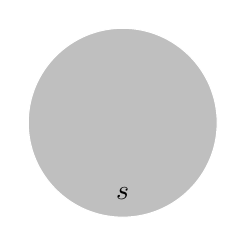
\begin{tikzpicture}
\filldraw[fill=gray!50, draw=white] (0, 0) circle (1.2);
\node at (0, -0.9) {$s$};
\end{tikzpicture}
\hspace{20pt}
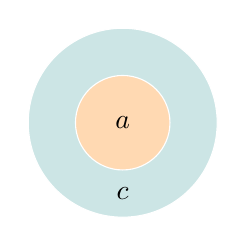
\begin{tikzpicture}
\filldraw[fill=blue!50!green!20, draw=white] (0, 0) circle (1.2);
\filldraw[fill=orange!30, draw=white] (0, 0) circle (0.6);
\node at (0, 0) {$a$};
\node at (0, -0.9) {$c$};
\end{tikzpicture}
\]

\hask{get}/\hask{set} 版本的透镜可以从这种存在形式中推导出来。
\begin{haskell}
toGet :: LensE s a -> (s -> a)
toGet (LensE (l, r)) = snd . l

toSet :: LensE s a -> (s -> a -> s)
toSet (LensE (l, r)) s a = r (fst (l s), a)
\end{haskell}

注意,我们不需要知道残差的类型。我们利用了存在性透镜同时包含 \hask{c} 的生产者和消费者这一事实,我们只是在两者之间进行调解。

无法提取“裸”残差,这由以下代码无法编译的事实证明:
\begin{haskell}
getResidue :: LensE s a -> c
getResidue (LensE (l, r)) = fst . l
\end{haskell}

\subsection{范畴论中的存在性透镜}

我们可以通过将存在类型表示为余积,轻松地将透镜的新定义翻译到范畴论中:
\[ \int^{c} \mathcal{C}(s, c \times a) \times  \mathcal{C}(c \times a, s) \]
事实上,我们可以将其推广到类型变化的透镜,其中焦点 $a$ 可以被替换为不同类型 $b$ 的新焦点。将 $a$ 替换为 $b$ 将产生一个新的复合对象 $t$:
\[
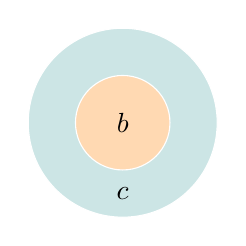
\begin{tikzpicture}
\filldraw[fill=blue!50!green!20, draw=white] (0, 0) circle (1.2);
\filldraw[fill=orange!30, draw=white] (0, 0) circle (0.6);
\node at (0, 0) {$b$};
\node at (0, -0.9) {$c$};
\end{tikzpicture}
\hspace{20pt}
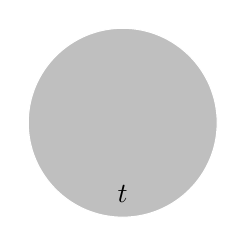
\begin{tikzpicture}
\filldraw[fill=gray!50, draw=white] (0, 0) circle (1.2);
\node at (0, -0.9) {$t$};
\end{tikzpicture}
\]

透镜现在由两对对象参数化:$\langle s, t\rangle$ 用于外部对象,$ \langle a, b \rangle$ 用于内部对象。存在性残差 $c$ 仍然隐藏:
\[ \mathcal{L}\langle s, t\rangle \langle a, b \rangle = \int^{c} \mathcal{C}(s, c \times a) \times  \mathcal{C}(c \times b, t) \]
余积下的积是 profunctor 的对角部分,它在 $y$ 中是协变的,在 $x$ 中是逆变的:
\[ \mathcal{C}(s, y \times a) \times  \mathcal{C}(x \times b, t) \]
\begin{exercise}
证明:
\[ \mathcal{C}(s, y \times a) \times  \mathcal{C}(x \times b, t) \]
是 $\langle x, y\rangle$ 中的 profunctor。
\end{exercise}

\subsection{Haskell 中的类型变化透镜}
在 Haskell 中,我们可以将类型变化透镜定义为以下 \index{存在性透镜}存在类型:
\begin{haskell}
data LensE s t a b where
  LensE :: (s -> (c, a)) -> ((c, b) -> t) -> LensE s t a b
\end{haskell}

与之前一样,我们可以使用存在性透镜来获取和设置焦点:
\begin{haskell}
toGet :: LensE s t a b -> (s -> a)
toGet (LensE l r) = snd . l

toSet :: LensE s t a b -> (s -> b -> t)
toSet (LensE l r) s a = r (fst (l s), a)
\end{haskell}

这两个函数,\hask{s->(c, a)} 和 \hask{(c, b)->t} 通常被称为 \emph{前向} 和 \emph{后向} 传递。
前向传递可用于提取焦点 \hask{a}。后向传递回答了以下问题:如果我们希望前向传递的结果是某个其他 \hask{b},我们应该传递什么 \hask{t} 给它?

有时我们只是在问:如果我们希望通过 \hask{b} 改变焦点,我们应该对输入进行什么改变 \hask{t}。后一种观点在使用透镜描述 \index{神经网络}神经网络时特别有用。

透镜的最简单示例作用于积。它可以提取或替换积的一个组件,将另一个组件视为残差。在 Haskell 中,我们将其实现为:
\begin{haskell}
prodLens :: LensE (c, a) (c, b) a b
prodLens = LensE id id
\end{haskell}
在这里,整体的类型是积 \hask{(c, a)}。当我们用 \hask{b} 替换 \hask{a} 时,我们最终得到目标类型 \hask{(c, b)}。由于源和目标已经是积,存在性透镜定义中的两个函数只是恒等函数。

\subsection{透镜组合}

使用透镜的主要优势在于它们可以组合。两个透镜的组合让我们可以放大组件的子组件。

假设我们从一个透镜开始,它允许我们访问焦点 \hask{a} 并将其更改为 \hask{b}。这个焦点是整体的一部分,由源 \hask{s} 和目标 \hask{t} 描述。

我们还有一个内部透镜,它可以访问 \hask{a} 内部的焦点 \hask{a'},并用 \hask{b'} 替换它,以给我们一个新的 \hask{b}。

我们现在可以构造一个复合透镜,它可以在 \hask{s} 和 \hask{t} 内部访问 \hask{a'} 和 \hask{b'}。关键在于我们意识到我们可以将两个残差的积作为新的残差:
\[
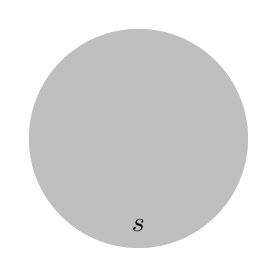
\begin{tikzpicture}
\filldraw[fill=gray!50, draw=white] (0, 0) circle (1.4);
\node at (0, -1.1) {$s$};
\end{tikzpicture}
\hspace{20pt}
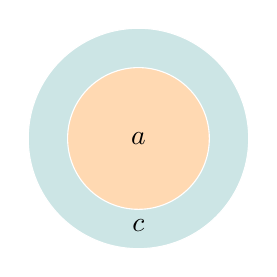
\begin{tikzpicture}
\filldraw[fill=blue!50!green!20, draw=white] (0, 0) circle (1.4);
\filldraw[fill=orange!30, draw=white] (0, 0) circle (0.9);
\node at (0, 0) {$a$};
\node at (0, -1.1) {$c$};
\end{tikzpicture}
\hspace{20pt}
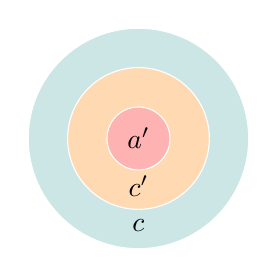
\begin{tikzpicture}
\filldraw[fill=blue!50!green!20, draw=white] (0, 0) circle (1.4);
\filldraw[fill=orange!30, draw=white] (0, 0) circle (0.9);
\filldraw[fill=red!30, draw=white] (0, 0) circle (0.4);
\node at (0, 0) {$a'$};
\node at (0, -0.6) {$c'$};
\node at (0, -1.1) {$c$};
\end{tikzpicture}
\]

\[
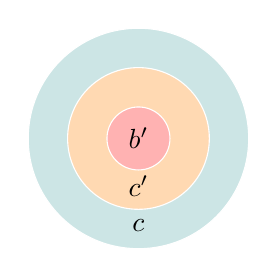
\begin{tikzpicture}
\filldraw[fill=blue!50!green!20, draw=white] (0, 0) circle (1.4);
\filldraw[fill=orange!30, draw=white] (0, 0) circle (0.9);
\filldraw[fill=red!30, draw=white] (0, 0) circle (0.4);
\node at (0, 0) {$b'$};
\node at (0, -0.6) {$c'$};
\node at (0, -1.1) {$c$};
\end{tikzpicture}
\hspace{20pt}
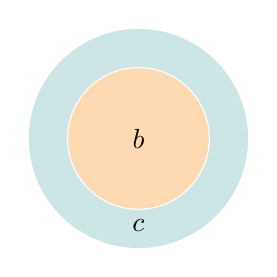
\begin{tikzpicture}
\filldraw[fill=blue!50!green!20, draw=white] (0, 0) circle (1.4);
\filldraw[fill=orange!30, draw=white] (0, 0) circle (0.9);
\node at (0, 0) {$b$};
\node at (0, -1.1) {$c$};
\end{tikzpicture}
\hspace{20pt}
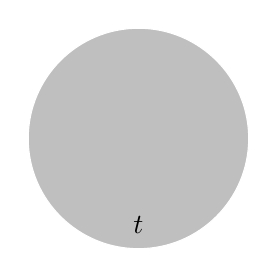
\begin{tikzpicture}
\filldraw[fill=gray!50, draw=white] (0, 0) circle (1.4);
\node at (0, -1.1) {$t$};
\end{tikzpicture}
\]

\begin{haskell}
compLens :: LensE a b a' b' -> LensE s t a b -> LensE s t a' b'
compLens (LensE l2 r2) (LensE l1 r1) = LensE l3 r3
  where l3 = assoc' . bimap id l2  . l1
        r3 = r1 . bimap id r2 . assoc
\end{haskell}
新透镜中的左映射由以下复合给出:
\[ s \xrightarrow{l_1} (c, a)   \xrightarrow{(id, l_2)} (c, (c', a'))  \xrightarrow{assoc'} ((c, c'), a')\]
右映射由以下复合给出:
\[ ((c, c'), b') \xrightarrow{assoc}  (c, (c', b')) \xrightarrow{(id, r_2)} (c, b) \xrightarrow{r_1} t \]

我们使用了积的结合性和函子性:
\begin{haskell}
assoc :: ((c, c'), b') -> (c, (c', b'))
assoc ((c, c'), b') = (c, (c', b'))

assoc' :: (c, (c', a')) -> ((c, c'), a')
assoc' (c, (c', a')) = ((c, c'), a')

instance Bifunctor (,) where
  bimap f g (a, b) = (f a, g b)
\end{haskell}

作为一个例子,让我们组合两个积透镜:
\begin{haskell}
l3 :: LensE (c, (c', a')) (c, (c', b')) a' b'
l3 = compLens prodLens prodLens
\end{haskell}
并将其应用于嵌套积:
\begin{haskell}
x :: (String, (Bool, Int))
x = ("Outer", (True, 42))
\end{haskell}
我们的复合透镜不仅允许我们检索最内层的组件:
\begin{haskell}
toGet l3 x
> 42
\end{haskell}
还可以用不同类型的值(这里是 \hask{Char})替换它:
\begin{haskell}
toSet l3 x 'z'
> ("Outer",(True,'z'))
\end{haskell}

\subsection{透镜的范畴}

由于透镜可以组合,你可能会想知道是否存在一个范畴,其中透镜是 hom-集。

确实,存在一个范畴 $\mathbf{Lens}$,其对象是 $\mathcal{C}$ 中的对象对,从 $\langle s, t\rangle$ 到 $ \langle a, b \rangle$ 的箭头是 $\mathcal{L} \langle s, t\rangle \langle a, b \rangle$ 的元素。

存在性透镜的组合公式过于复杂,无法在实践中使用。在下一章中,我们将看到使用 Tambara 模块的透镜的另一种表示,其中组合只是函数的组合。

\section{透镜与纤维化}

使用纤维丛的语言,我们可以从另一个角度来理解透镜。定义纤维化的投影 $p$ 可以被视为将丛 $E$ "分解" 为纤维。

在这种视角下,$p$ 扮演了 \hask{get} 的角色:
\[ p \colon E \to B \]
其中基空间 $B$ 表示焦点的类型,而 $E$ 表示可以从中提取该焦点的复合类型。

透镜的另一部分,\hask{set},是一个映射:
\[ q \colon E \times B \to E \]
让我们看看如何用纤维化来解释它。
\subsection{传输律}

我们将 $q$ 解释为将丛 $E$ 中的一个元素"传输"到一个新的纤维。新的纤维由 $B$ 中的一个元素指定。

这种传输的性质由 get/set 透镜律,或称\emph{传输}律表达,它表示"你设置的就是你得到的":
\begin{haskell}
get (set s a) = a
\end{haskell}
我们说 $q(s, a)$ 将 $s$ 传输到 $a$ 上的新纤维:

\[
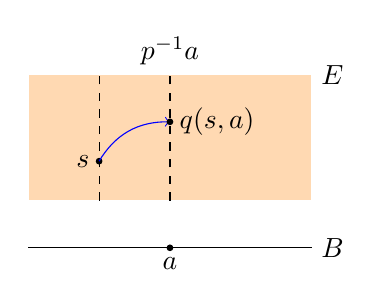
\begin{tikzpicture}

\def\yb{0}; % base
\def\yfb{0.6}; % fiber bottom
\def\yfs{1.1}; % s
\def\yfss{1.6}; % s'
\def\yft{2.2}; % fiber top

\def\dx{0.9};

\def\xbl{0};
\def\xbm{\xbl + \dx};
\def\xbmr{\xbl + 2*\dx};
\def\xbr{\xbl + 4*\dx};


\filldraw[fill=orange!30, draw=white] (\xbl, \yfb) rectangle (\xbr, \yft);

\draw (\xbl, \yb) -- (\xbr, \yb);

\draw[dashed] (\xbm, \yfb) -- (\xbm, \yft); %fiber
\draw[dashed] (\xbmr, \yfb) -- (\xbmr, \yft); %fiber

\filldraw[black] (\xbm, \yfs) circle (1 pt);
\node[left] at (\xbm, \yfs) {$s$};
\draw[blue] (\xbm, \yfs) edge[->, bend left] (\xbmr, \yfss);
\filldraw[black] (\xbmr, \yfss) circle (1 pt);
\node[right] at (\xbmr, \yfss) {$q(s, a)$};

\filldraw[black] (\xbmr, \yb) circle (1 pt);
\node[below] at (\xbmr, \yb) {$a$};

\node[above] at (\xbmr, \yft) {$p^{-1} a$};
\node[right] at (\xbr, \yb) {$B$};
\node[right] at (\xbr, \yft) {$E$};

\end{tikzpicture}
\]

我们可以用 $p$ 和 $q$ 重写这个定律:
\[ p \circ q = \pi_2 \]
其中 $\pi_2$ 是积的第二个投影。

等价地,我们可以将其表示为交换图:
\[
 \begin{tikzcd}
 E \times B
 \arrow[dd, "\varepsilon \times id"']
 \arrow[rd, "q"]
 \\
 & E
 \arrow[dl, "p"]
 \\
 B
  \end{tikzcd}
\]
这里,我没有使用投影 $\pi_2$,而是使用了余幺半群的余单位 $\varepsilon$:
\[ \varepsilon \colon E \to 1 \]
然后遵循积的单位律。使用余幺半群使得将这个构造推广到幺半范畴中的张量积更加容易。

\subsection{恒等律}
这是 set/get 律,或称\emph{恒等}律。它表示"如果你设置你得到的,那么什么都不会改变":
\begin{haskell}
set s (get  s) = s
\end{haskell}
我们可以用余幺半群的余乘法来表示它:
\[ \delta \colon E \to E \times E \]
set/get 律要求以下复合是恒等的:
\[ E \xrightarrow{\delta} E \times E \xrightarrow{id \times p} E \times B \xrightarrow{q} E \]
这是该定律在丛中的图示:
\[
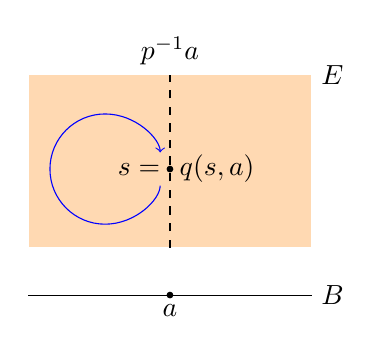
\begin{tikzpicture}

\def\yb{0}; % base
\def\yfb{0.6}; % fiber bottom
\def\yfs{1.1}; % s
\def\yfss{1.6}; % s'
\def\yft{2.8}; % fiber top

\def\dx{0.9};

\def\xbl{0};
\def\xbm{\xbl + \dx};
\def\xbmr{\xbl + 2*\dx};
\def\xbr{\xbl + 4*\dx};


\filldraw[fill=orange!30, draw=white] (\xbl, \yfb) rectangle (\xbr, \yft);

\draw (\xbl, \yb) -- (\xbr, \yb);

\draw[dashed] (\xbmr, \yfb) -- (\xbmr, \yft); %fiber

\node at (\xbmr, \yfss) (s) {};
\draw[->,shorten <=6pt,shorten >=6pt, blue](s.west)arc(360:0:0.7);
\filldraw[black] (\xbmr, \yfss) circle (1 pt);
\node[left] at (\xbmr, \yfss) {$s = $};
\node[right] at (\xbmr, \yfss) {$q(s, a)$};

\filldraw[black] (\xbmr, \yb) circle (1 pt);
\node[below] at (\xbmr, \yb) {$a$};

\node[above] at (\xbmr, \yft) {$p^{-1} a$};
\node[right] at (\xbr, \yb) {$B$};
\node[right] at (\xbr, \yft) {$E$};

\end{tikzpicture}
\]

\subsection{复合律}

最后,这是 set/set 律,或称\emph{复合}律。它表示"最后的设置胜出":
\begin{haskell}
set (set s a) a' = set s a'
\end{haskell}
以及相应的交换图:
\[
 \begin{tikzcd}
 E \times B \times B
 \arrow[d, "id \times \varepsilon \times id"']
 \arrow[rd, "q \times id"]
 \\
 E \times B
 \arrow[d, "q"']
 & E \times B
 \arrow[dl, "q "]
 \\
 E
  \end{tikzcd}
\]
同样,为了去掉中间的 $B$,我使用了余单位而不是积的投影。

这是 set/set 律在丛中的图示:
\[
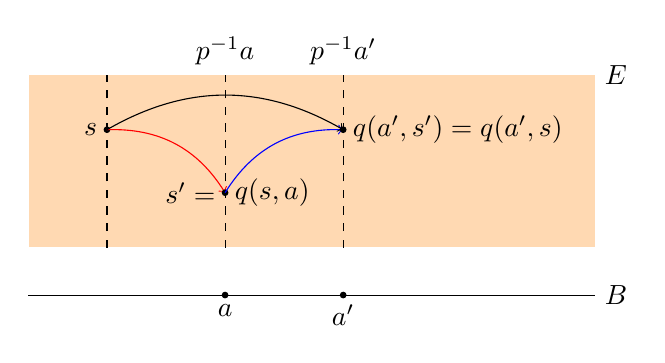
\begin{tikzpicture}

\def\yb{0}; % base
\def\yfb{0.6}; % fiber bottom
\def\yfs{1.3}; % s'
\def\yfss{2.1}; % s''
\def\yft{2.8}; % fiber top

\def\dx{1};

\def\xbl{0};
\def\xbm{\xbl + \dx};
\def\xbmr{\xbl + 2.5*\dx};
\def\xbmrr{\xbl + 4*\dx};
\def\xbr{\xbl + 7.2*\dx};


\filldraw[fill=orange!30, draw=white] (\xbl, \yfb) rectangle (\xbr, \yft);

\draw (\xbl, \yb) -- (\xbr, \yb);

\draw[dashed] (\xbm, \yfb) -- (\xbm, \yft); %fiber
\draw[dashed] (\xbmr, \yfb) -- (\xbmr, \yft); %fiber
\draw[dashed] (\xbmrr, \yfb) -- (\xbmrr, \yft); %fiber

\filldraw[black] (\xbm, \yfss) circle (1 pt);
\node[left] at (\xbm, \yfss) {$s$};

\draw[red] (\xbm, \yfss)  edge[->, bend left]  (\xbmr, \yfs);

\filldraw[black] (\xbmr, \yfs) circle (1 pt);
\node[right] at (\xbmr, \yfs) {$q(s, a)$};
\node[left] at (\xbmr, \yfs) {$s' =$};

\draw[blue] (\xbmr, \yfs) edge[->, bend left] (\xbmrr, \yfss);

\filldraw[black] (\xbmrr, \yfss) circle (1 pt);
\node[right] at (\xbmrr, \yfss) {$q(a', s') = q(a', s)$};

\draw (\xbm, \yfss) edge[->, bend left] (\xbmrr, \yfss);


\filldraw[black] (\xbmr, \yb) circle (1 pt);
\node[below] at (\xbmr, \yb) {$a$};

\filldraw[black] (\xbmrr, \yb) circle (1 pt);
\node[below] at (\xbmrr, \yb) {$a'$};

\node[above] at (\xbmr, \yft) {$p^{-1} a$};
\node[above] at (\xbmrr, \yft) {$p^{-1} a'$};
\node[right] at (\xbr, \yb) {$B$};
\node[right] at (\xbr, \yft) {$E$};

\end{tikzpicture}
\]

\subsection{类型转换透镜}

类型转换透镜将传输推广到在丛之间进行。我们必须定义一整个丛族。我们从范畴 $\cat A$ 开始,其对象定义了我们将用于透镜焦点的类型。

我们将集合 $B$ 构造为所有焦点类型的所有元素的并集。$B$ 在 $\cat A$ 上纤维化——投影 $\pi$ 将 $B$ 中的一个元素发送到其对应的类型。你可以将 $B$ 视为余切片范畴 $1/ \cat A$ 的对象集。

丛的丛 $E$ 是一个在 $B$ 上纤维化的集合,投影为 $p$。由于 $B$ 本身在 $\cat A$ 上纤维化,$E$ 传递地在 $\cat A$ 上纤维化,复合投影为 $\pi \circ p$。正是这种较粗的纤维化将 $E$ 分解为一系列丛。每个丛对应于给定焦点类型的复合类型的不同类型。类型转换透镜将在这些丛之间移动。

\[
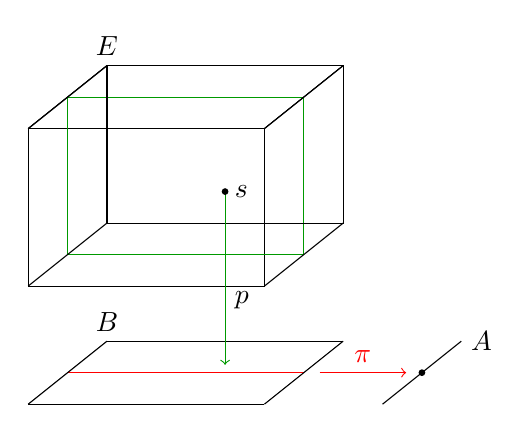
\begin{tikzpicture}
\def\xl{-3};
\def\xr{0};
\def\yb{0};
\def\yt{2};

\def\dy{0.4};
\def\dx{0.5};

\def\a{(\xl, \yb)};
\def\b{(\xr, \yb)};
\def\c{(\xl, \yt)};
\def\d {(\xr, \yt)};

% _a second plane
\def\aa{(\xl + \dx, \yb + \dy)};
\def\ba{(\xr + \dx, \yb + \dy)};
\def\ca{(\xl + \dx, \yt + \dy)};
\def\da{(\xr + \dx, \yt + \dy)};

% _b third plane
\def\ab{(\xl + 2*\dx, \yb + 2*\dy)};
\def\bb{(\xr + 2*\dx, \yb + 2*\dy)};
\def\cb{(\xl + 2*\dx, \yt + 2*\dy)};
\def\db{(\xr + 2*\dx, \yt + 2*\dy)};

% shifted walls
\def\yshift{-1.5};
\def\xshift{1.5};

% E
\draw \a rectangle \d;
\draw[draw=black!40!green] \aa rectangle \da;
\draw \ab rectangle \db;

\draw \a -- \ab;
\draw \b -- \bb;
\draw \d -- \db;
\draw \c -- \cb;

\node[above] at \cb {$E$};

% B
% rebase yb (bottom)
\def\yb{\yshift}
% rebase xr (right wall)
\def\xr{0};

\draw \a -- \b;
\draw \ab -- \bb;
\draw[red] \aa -- \ba;
% diagonal
\draw \a -- \ab;
\draw \b -- \bb;
\draw \d -- \db;
\draw \c -- \cb;
\node[above] at \ab {$B$};


% A
% rebase yb (bottom)
\def\yb{\yshift}
% rebase xr (right wall)
\def\xr{\xshift};

\draw \b -- \bb;
\node[right] at \bb {$\cat A$};
\filldraw[black] \ba circle (1 pt);

%projections

\draw[red, shorten <=0.2cm, shorten >=0.2cm, ->] (0 + \dx, \yshift + \dy) -- node[above]{$\pi$} (\xshift +\dx, \yshift + \dy);

\draw[draw=black!40!green, shorten >=0.1cm, ->] (0 - \dx, 0 + 3 * \dy) -- node[below right]{$p$} (0 - \dx, \yshift + \dy);

\node[right] at (0 - \dx, 0 + 3 * \dy) {$s$};
\filldraw[black] (0 - \dx, 0 + 3 * \dy) circle (1 pt);


\end{tikzpicture}
\]

投影 $p$ 取一个元素 $s \in E$ 并生成一个元素 $b \in B$,其类型由 $\pi b$ 给出。这是 \hask{get} 的推广。

传输 $q$,对应于 \hask{set},取一个元素 $s \in E$ 和一个元素 $b \in B$ 并生成一个新元素 $t \in E$。重要的观察是 $s$ 和 $t$ 可能属于 $E$ 的不同子丛。

传输满足以下定律:

get/set 律(传输):

\[ p (q (b, s)) = b \]

set/get 律(恒等):

\[ q ( p (s), s) = s \]

set/set 律(复合):

\[ q (c, q (b, s)) = q (c, s) \]

\section{重要公式}
这是一个方便的(余)端演算速查表。
\begin{itemize}
\item 同态函子的连续性:
\[\cat D\left(d, \int_a P\langle a, a \rangle \right) \cong \int_a \cat D \left(d, P\langle a, a \rangle \right) \]
\item 同态函子的余连续性:
\[\cat D\left( \int^a P\langle a, a \rangle , d \right) \cong \int_a \cat D \left( P\langle a, a \rangle, d \right) \]
\item 忍者米田引理:
\[ \int_{x} \mathbf{Set} (\mathcal{C}(a, x), F x) \cong F a \]
\item 忍者余米田引理:
\[ \int^{x} \mathcal{C}(x, a) \times F x \cong F a \]
\item 逆变函子(预层)的忍者米田引理:
\[ \int_{x} \mathbf{Set} (\mathcal{C}(x, a), G x) \cong G a \]
\item 逆变函子的忍者余米田引理:
\[ \int^{x} \mathcal{C}(a, x) \times G x \cong G a \]
\item Day卷积:
\[ (F \star G) x = \int^{a, b} \cat C (a \otimes b, x) \times F a \times G b \]

\end{itemize}


\end{document}